
% ============================================================
% Additional Material
% ============================================================
\begin{frame}[c]
    \centering

    \vfill

    {\LARGE\bfseries Additional Material}

    \vspace{0.35cm}

    {\small Backup Slides}

    \vfill
\end{frame}

% ============================================================
%  Droplet-Diameter Sensitivity
% ============================================================

\begin{frame}{\small  Water-Mass Variability by Droplet Diameter (15 Bins)}
\scriptsize

\vspace{-0.3cm}

\begin{columns}[T,onlytextwidth]

\begin{column}{0.50\textwidth}
    \centering
    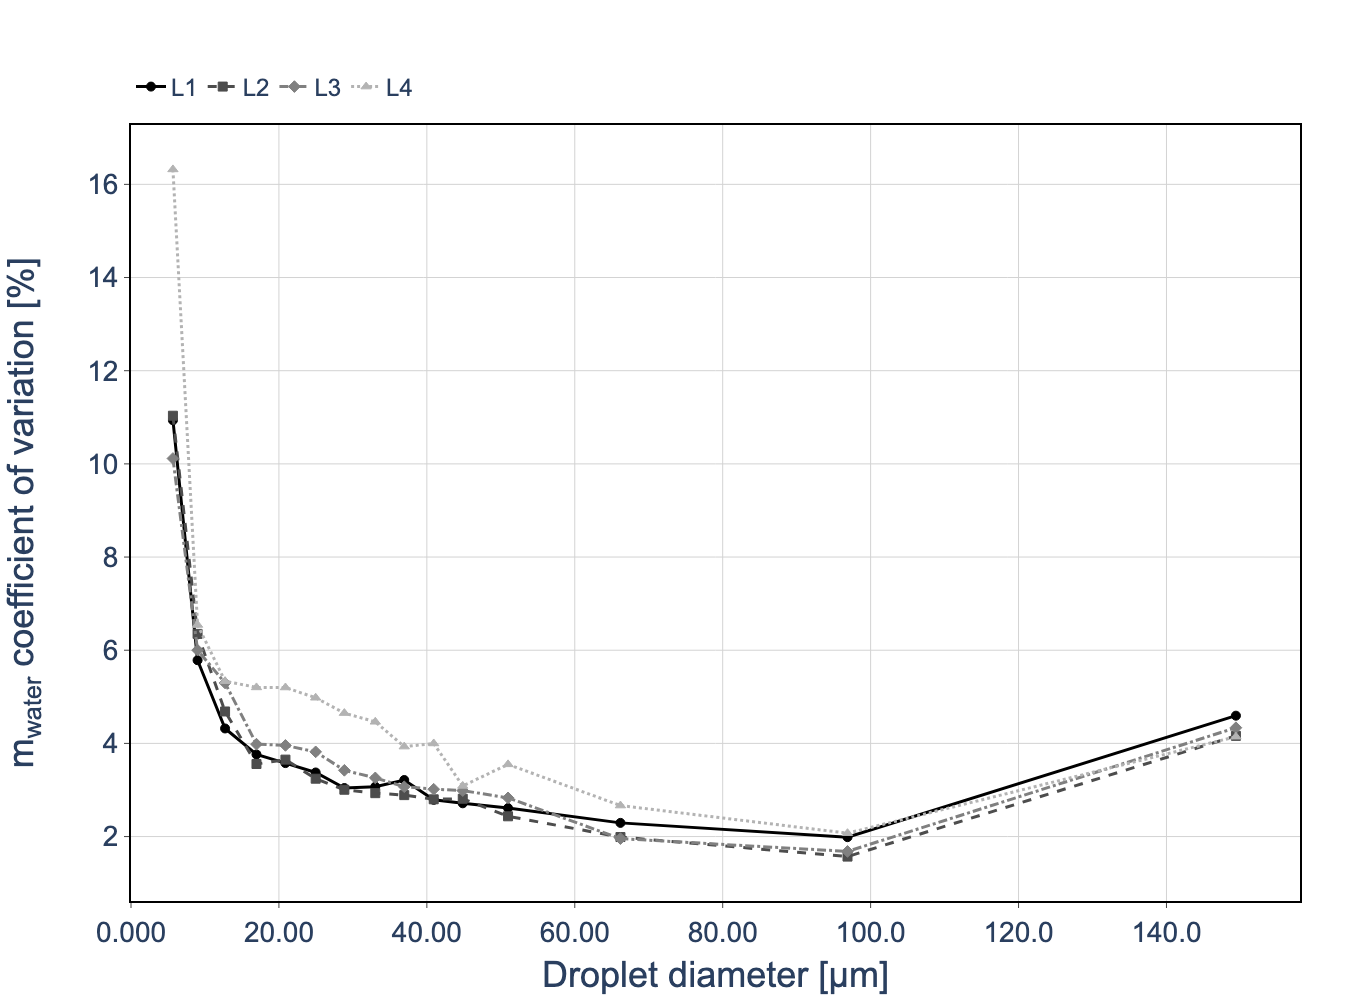
\includegraphics[trim={0cm 0cm 1cm 2.6cm}, clip, width=0.98\textwidth]{FIGURES/IMPINGEMENT/tc_naca0012_ae3932_water_mass_coefficient_of_variation_vs_droplet_diameter_bins15_all_grid_levels.png}
    \textbf{Coefficient of Variation}
\end{column}

\begin{column}{0.50\textwidth}
    \centering
    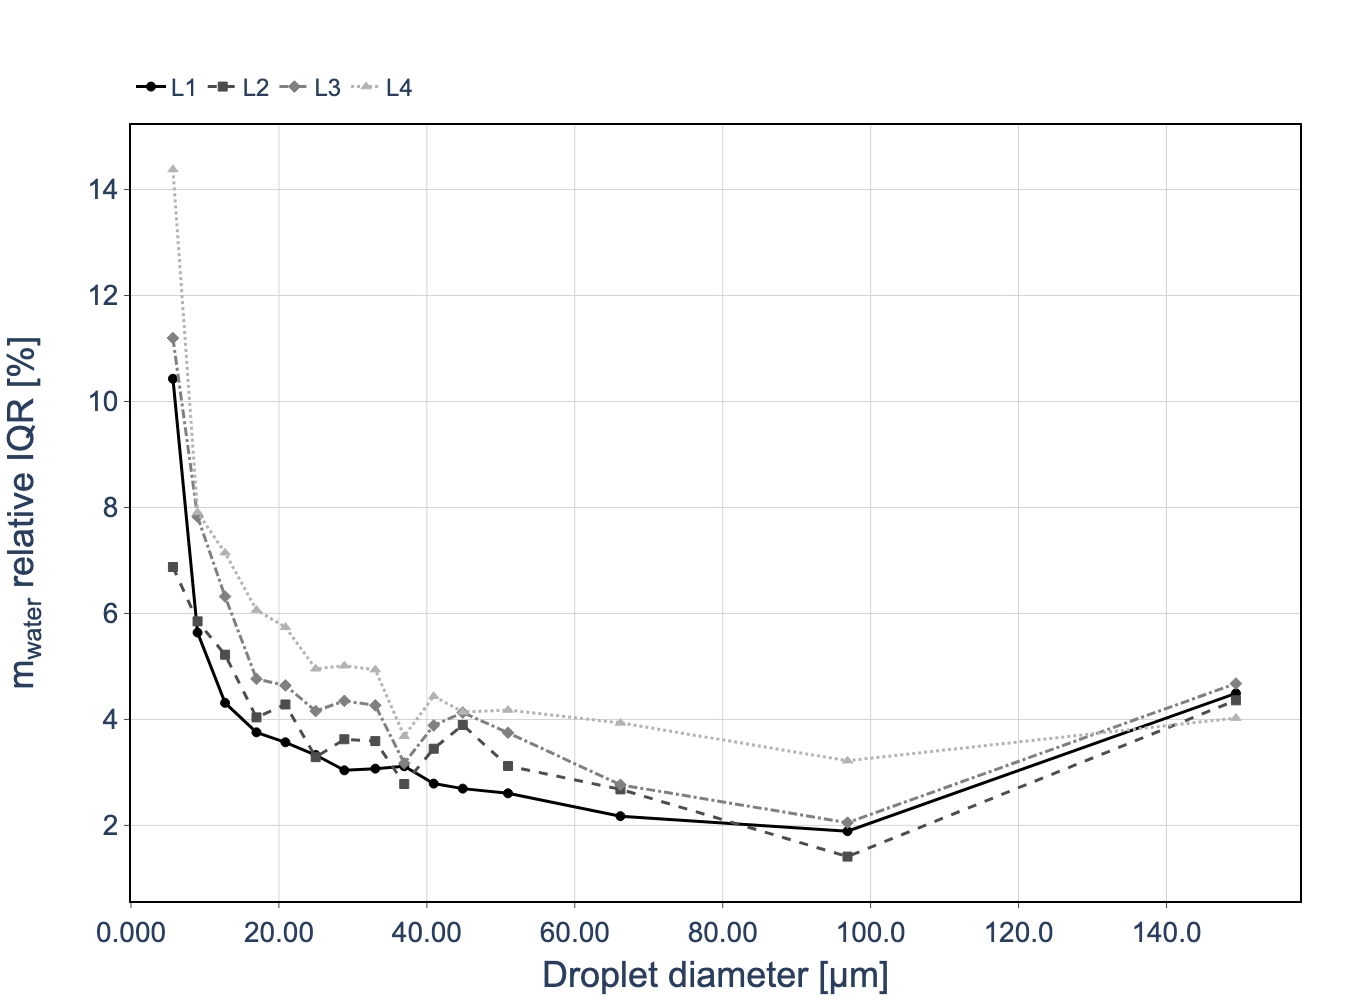
\includegraphics[trim={0cm 0cm 1cm 2.6cm}, clip, width=0.98\textwidth]{FIGURES/IMPINGEMENT/tc_naca0012_ae3932_water_mass_relative_iqr_vs_droplet_diameter_bins15_all_grid_levels.png}
    \textbf{Relative IQR}
\end{column}

\end{columns}

\vspace{-0.15cm}

\begin{block}{\scriptsize Observations}
\begin{itemize}
    \item Variability is evaluated from the optionally submitted water mass per droplet diameter, across all available participants and grid levels.
    \item Code-to-code variability is greatest for the smallest droplets and lowest across intermediate diameters.
    \item Coarser grids generally show greater spread.
\end{itemize}
\end{block}

\end{frame}

% ============================================================
% NACA0012 -- Surface Temperature by Thermodynamic Model
% ============================================================

\begin{frame}{\small NACA0012 -- Surface Temperature by Thermodynamic Model}
\scriptsize

\vspace{-0.15cm}

\begin{columns}[T,onlytextwidth]

% ------------------------------------------------------------
% AE3932
% ------------------------------------------------------------
\begin{column}{0.49\textwidth}
    \centering
    \textbf{AE3932}

    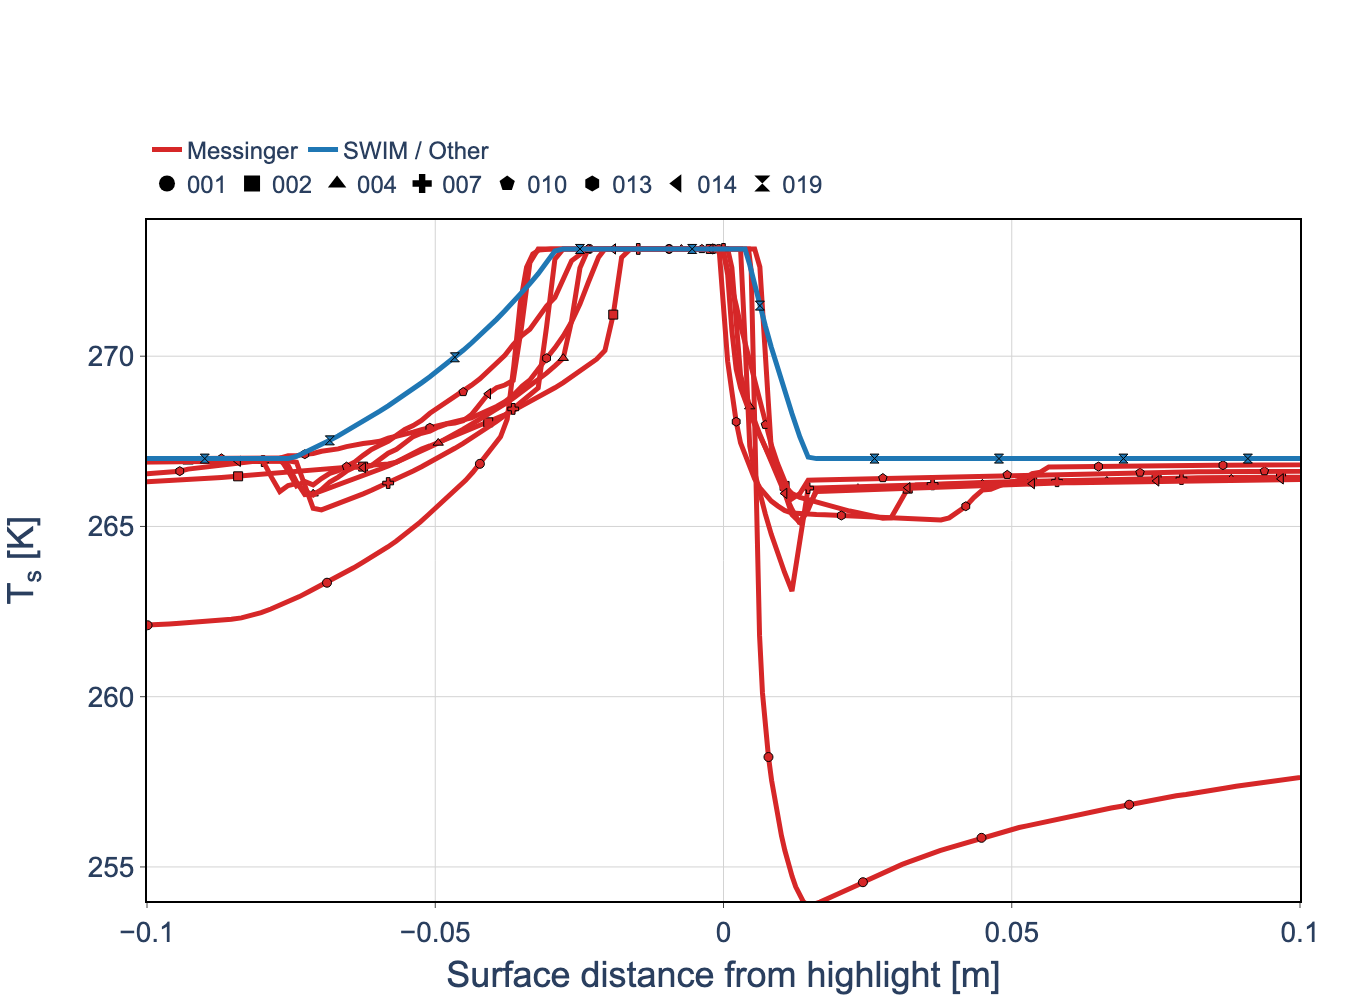
\includegraphics[
        width=\textwidth,
        keepaspectratio
    ]{FIGURES/SURF_TEMP_FF/tc_naca0012_ae3932_L1_surface_temperature_vs_s_slice_0p9144_grouped_thermodynamics_models.png}
\end{column}

% ------------------------------------------------------------
% AE3933
% ------------------------------------------------------------
\begin{column}{0.49\textwidth}
    \centering
    \textbf{AE3933}

    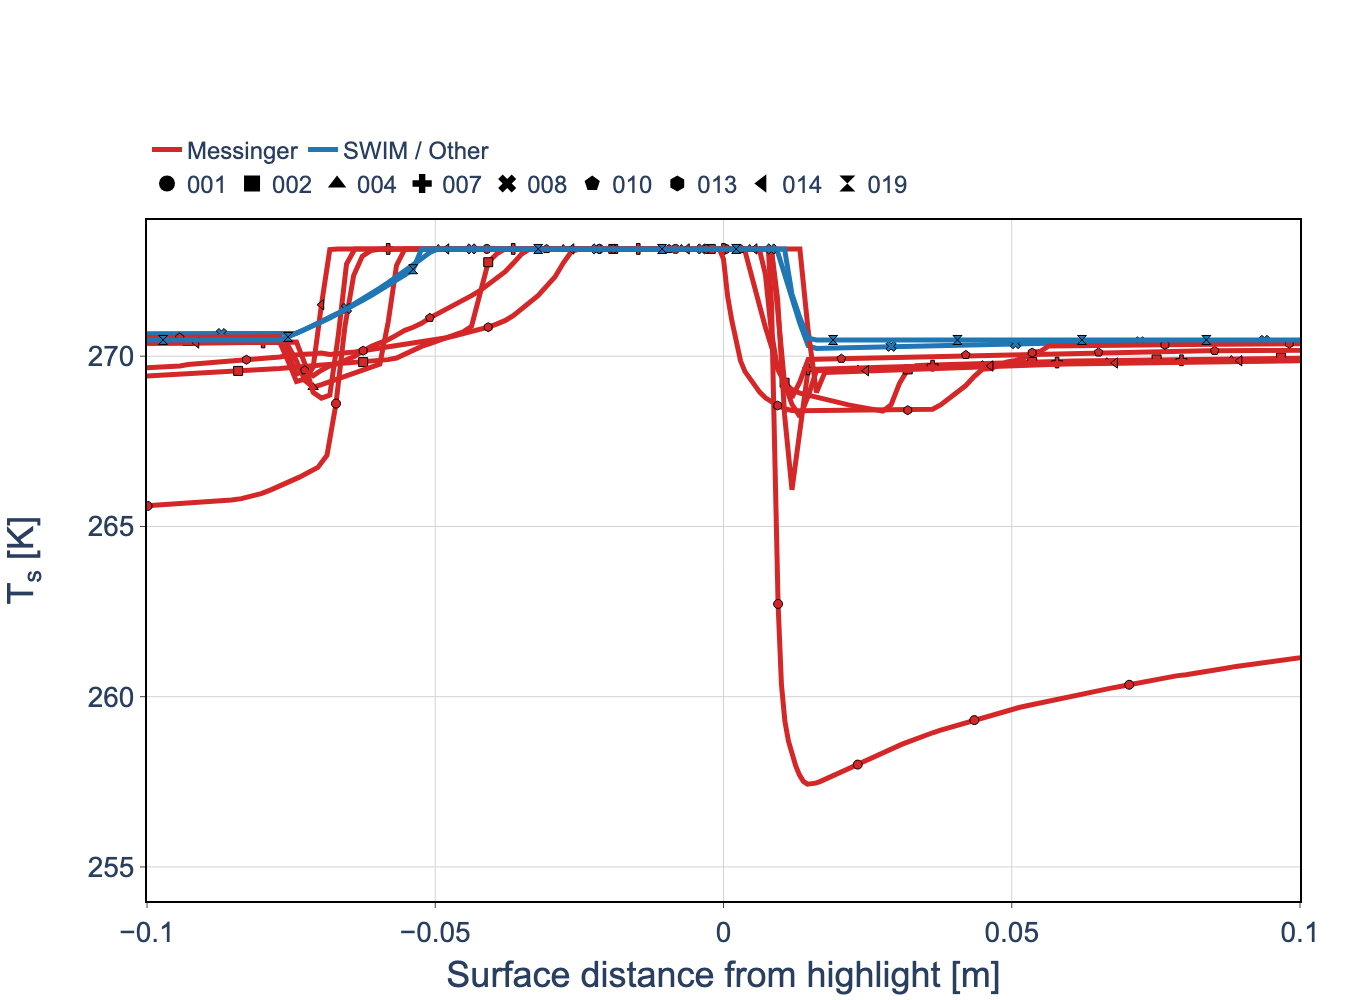
\includegraphics[
        width=\textwidth,
        keepaspectratio
    ]{FIGURES/SURF_TEMP_FF/tc_naca0012_ae3933_L1_surface_temperature_vs_s_slice_0p9144_grouped_thermodynamics_models.png}
\end{column}

\end{columns}

\end{frame}


% ============================================================
% NACA0012 -- Mean Surface Temperature
% ============================================================

\begin{frame}{\small NACA0012 -- Mean Surface Temperature}
\scriptsize

\vspace{-0.15cm}

\begin{columns}[T,onlytextwidth]

% ------------------------------------------------------------
% AE3932
% ------------------------------------------------------------
\begin{column}{0.49\textwidth}
    \centering
    \textbf{AE3932}

    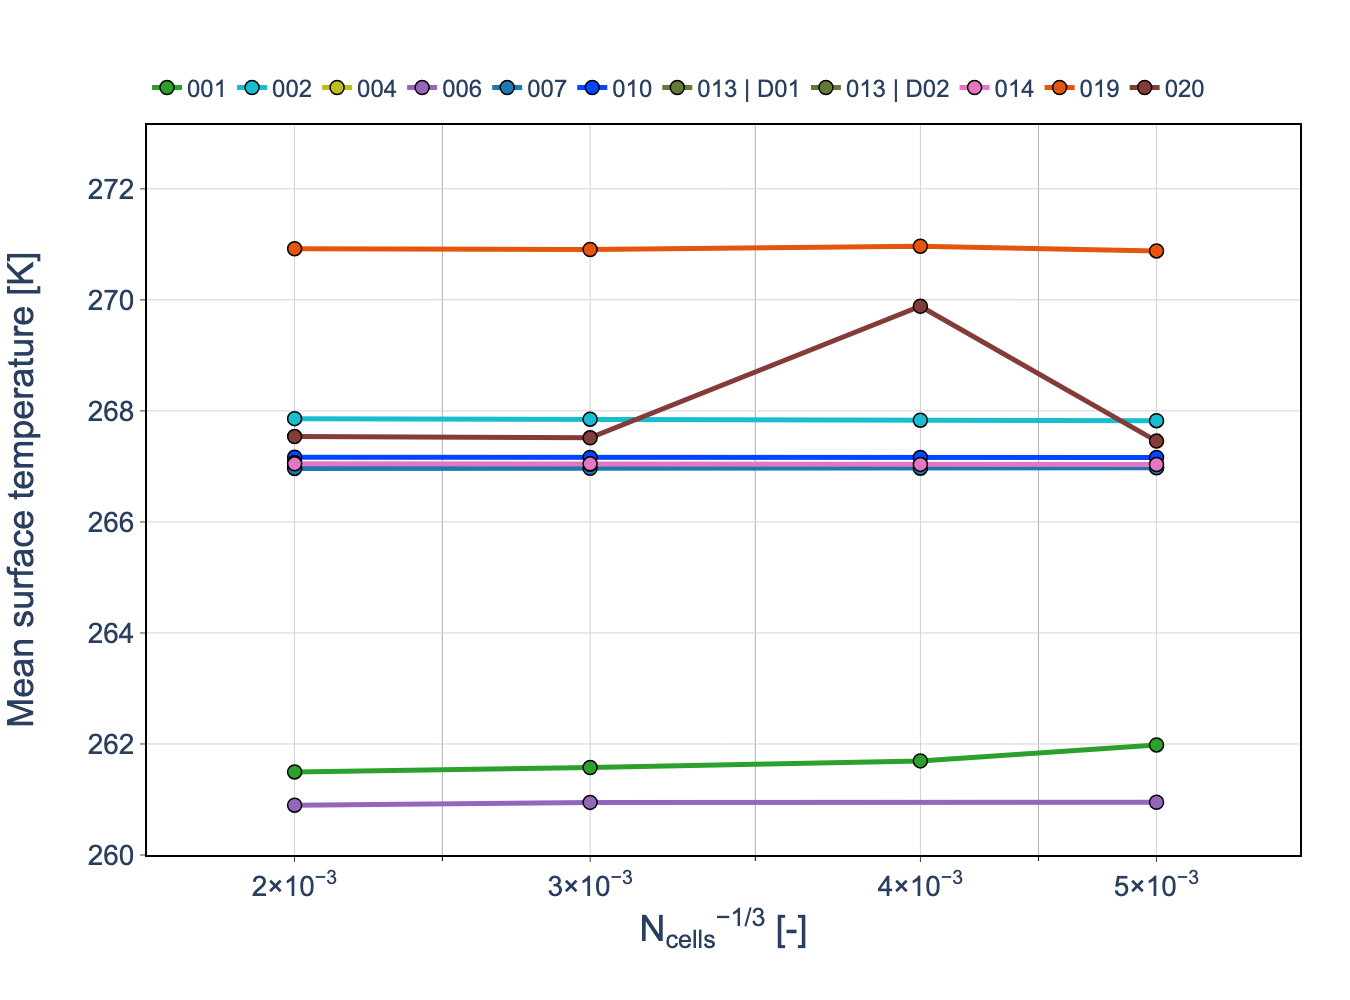
\includegraphics[
        width=\textwidth,
        keepaspectratio
    ]{FIGURES/SURF_TEMP_FF/tc_naca0012_ae3932_mean_surface_temperature_vs_n_slice_0p9144_all_roughness.png}
\end{column}

% ------------------------------------------------------------
% AE3933
% ------------------------------------------------------------
\begin{column}{0.49\textwidth}
    \centering
    \textbf{AE3933}

    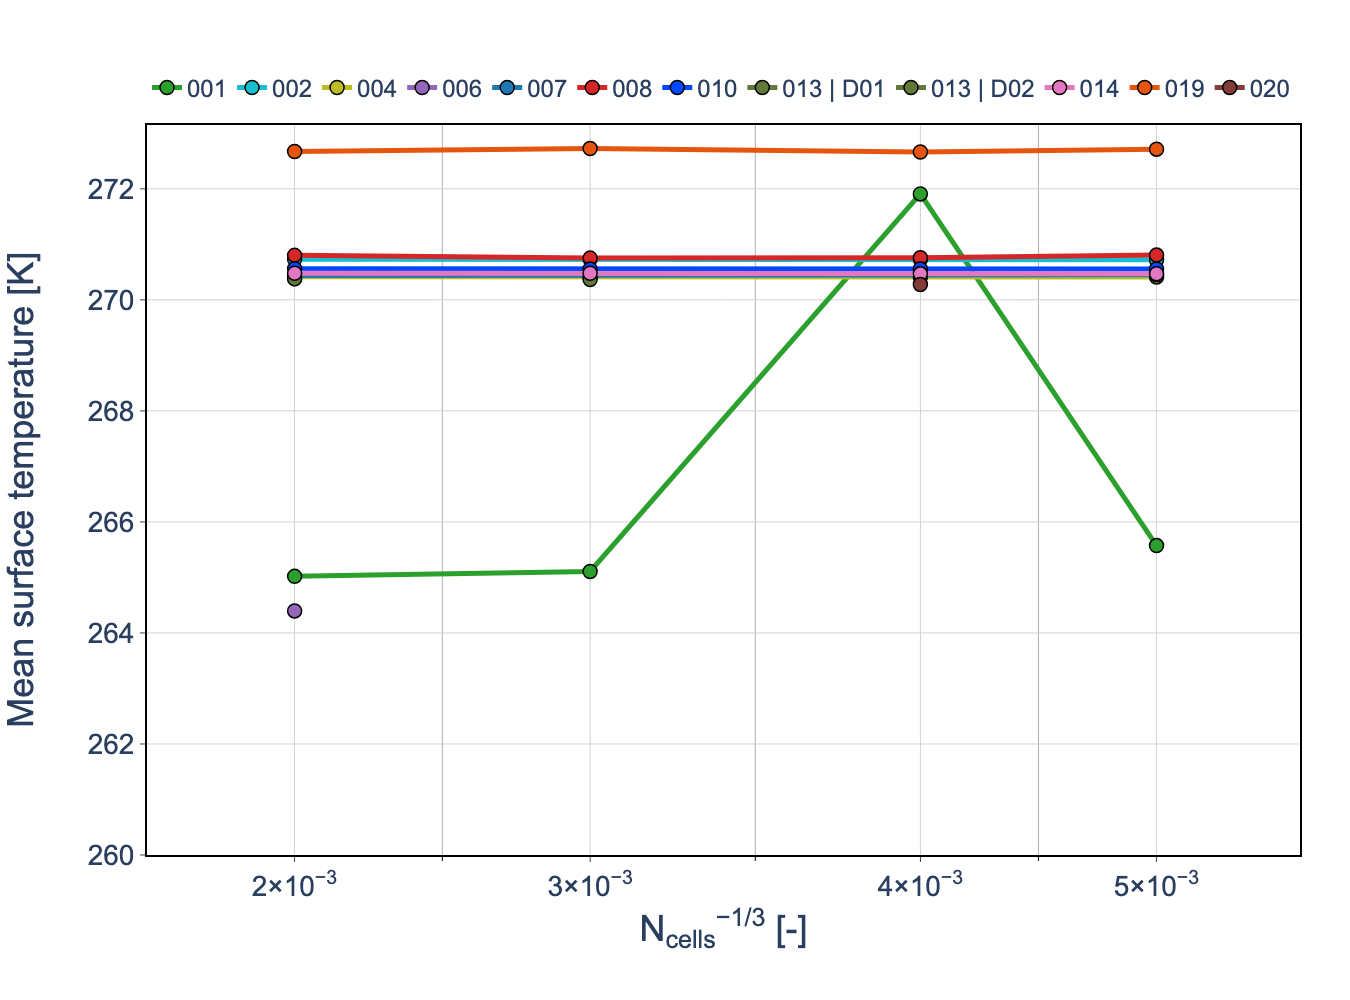
\includegraphics[
        width=\textwidth,
        keepaspectratio
    ]{FIGURES/SURF_TEMP_FF/tc_naca0012_ae3933_mean_surface_temperature_vs_n_slice_0p9144_all_roughness.png}
\end{column}

\end{columns}

\vspace{0.10cm}

\centering
{\tiny\textit{Note: Mean surface temperature is computed only over regions with ice thickness $> 0$.}}

\end{frame}

% ============================================================
% NACA0012 -- Freezing Fraction by Thermodynamic Model
% ============================================================

\begin{frame}{\small NACA0012 -- Freezing Fraction by Thermodynamic Model}
\scriptsize

\vspace{-0.15cm}

\begin{columns}[T,onlytextwidth]

% ------------------------------------------------------------
% AE3932
% ------------------------------------------------------------
\begin{column}{0.49\textwidth}
    \centering
    \textbf{AE3932}

    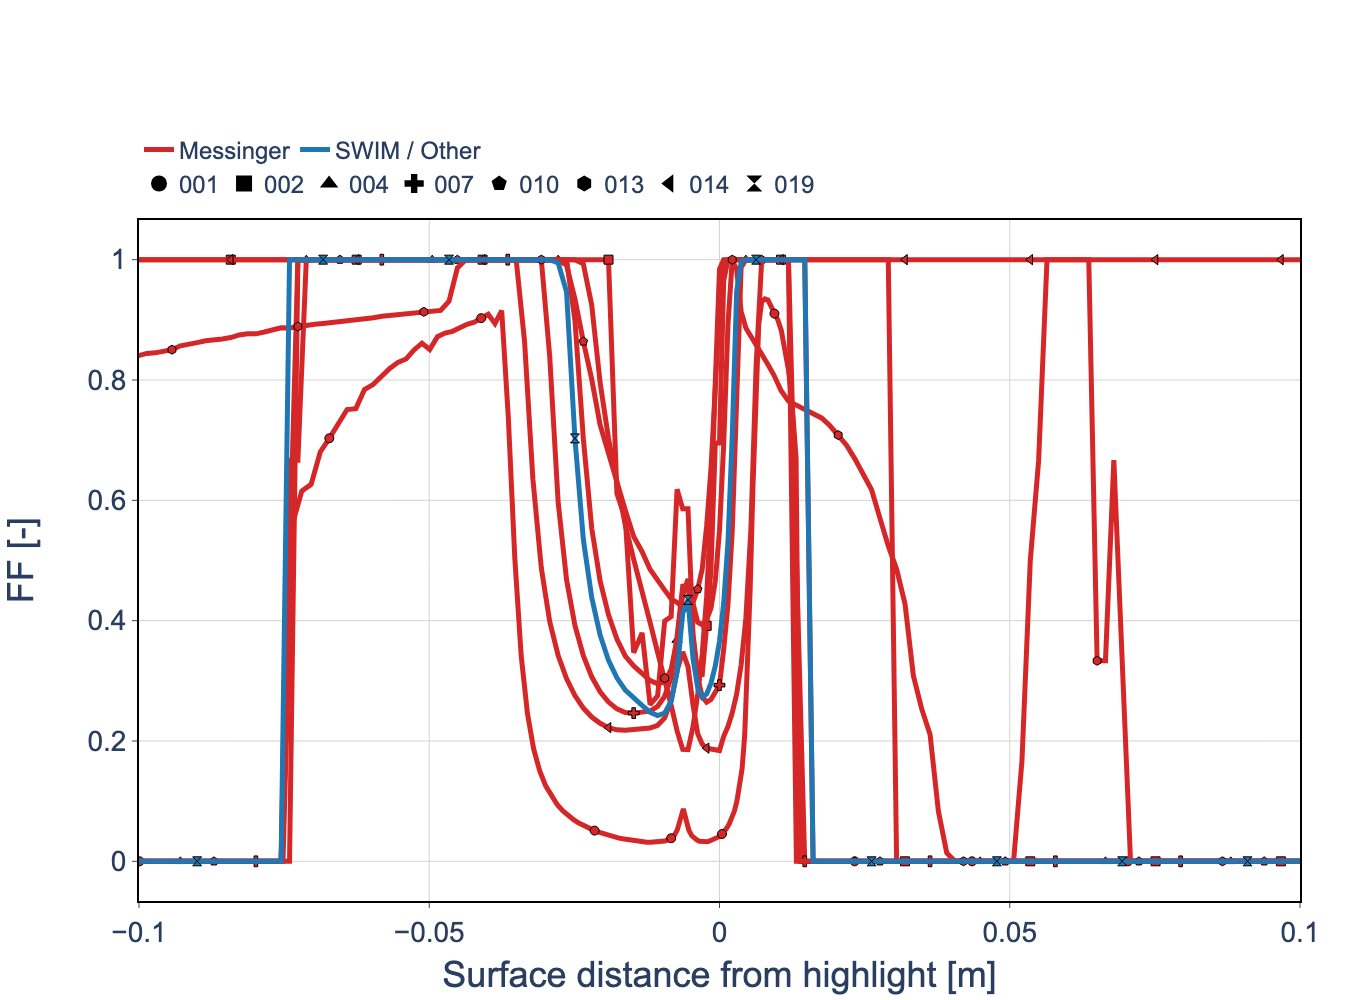
\includegraphics[
        width=\textwidth,
        keepaspectratio
    ]{FIGURES/SURF_TEMP_FF/tc_naca0012_ae3932_L1_freezing_fraction_vs_s_slice_0p9144_grouped_thermodynamics_models.png}
\end{column}

% ------------------------------------------------------------
% AE3933
% ------------------------------------------------------------
\begin{column}{0.49\textwidth}
    \centering
    \textbf{AE3933}

    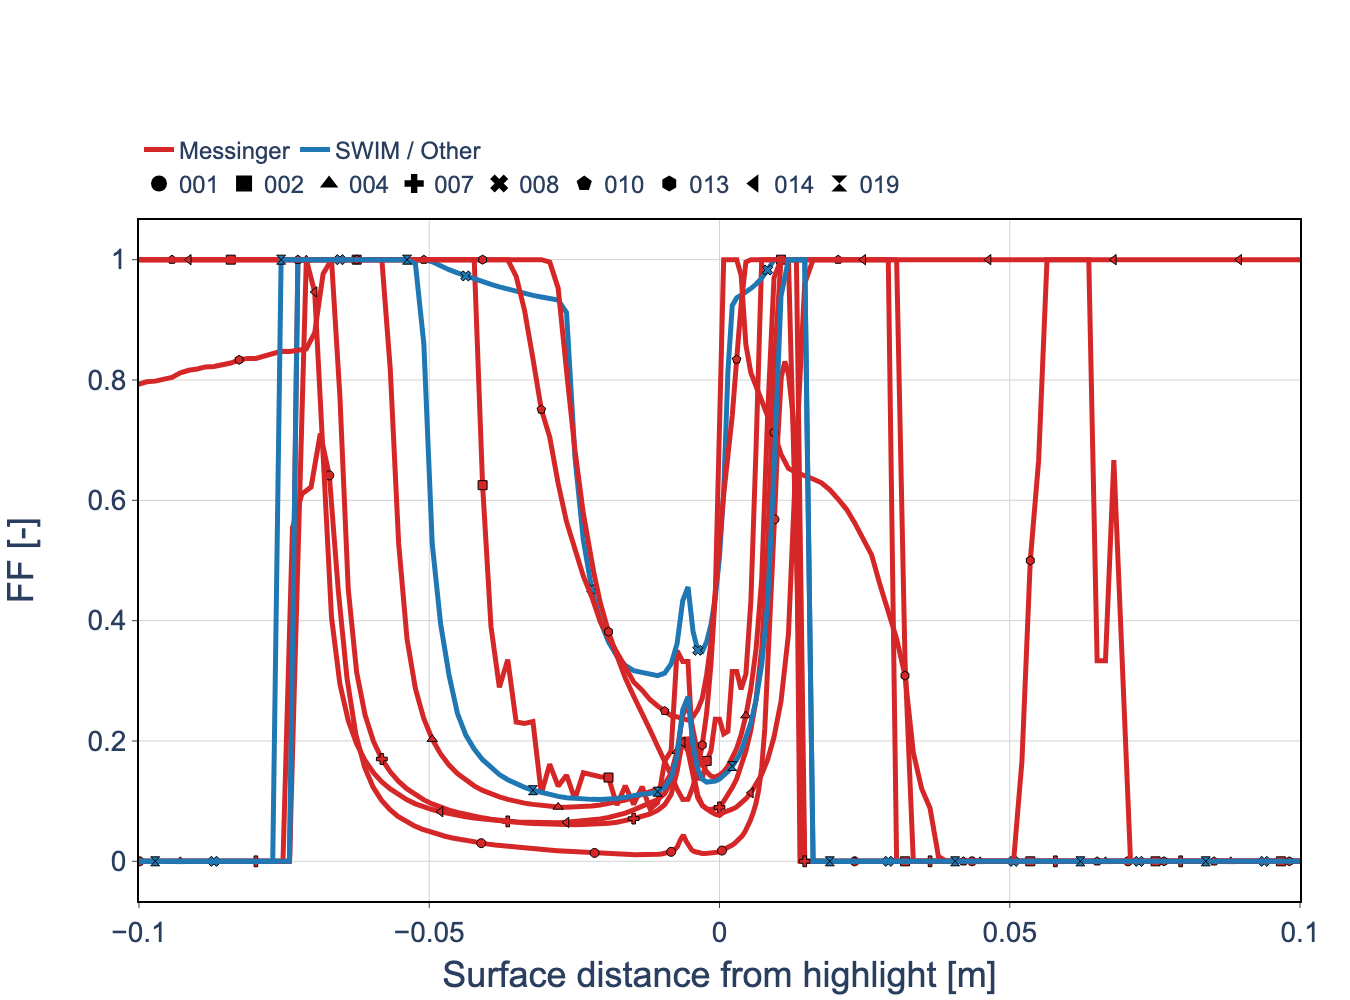
\includegraphics[
        width=\textwidth,
        keepaspectratio
    ]{FIGURES/SURF_TEMP_FF/tc_naca0012_ae3933_L1_freezing_fraction_vs_s_slice_0p9144_grouped_thermodynamics_models.png}
\end{column}

\end{columns}

\end{frame}

% ============================================================
%  Ice Mass Difference Between Conditions
% ============================================================

\begin{frame}{\small  Ice Mass Difference Between Conditions (15 Bins)}
\scriptsize

\begin{columns}[T,onlytextwidth]

% ------------------------------------------------------------
% Absolute difference
% ------------------------------------------------------------
\begin{column}{0.50\textwidth}
    \centering
    
\includegraphics[trim={0cm 1cm 1cm 2.6cm}, clip, width=\textwidth]{%
    FIGURES/ICE_ACCRETION/tc_naca0012_ae3933_comparison_with_3932_ice_mass_bins15_difference.png}

    \vspace{0.03cm}
    {\scriptsize\textbf{AE3933 $-$ AE3932}}
\end{column}

% ------------------------------------------------------------
% Percentage difference
% ------------------------------------------------------------
\begin{column}{0.50\textwidth}
    \centering
    
\includegraphics[trim={0cm 1cm 1cm 2.6cm}, clip, width=\textwidth]{%
    FIGURES/ICE_ACCRETION/tc_naca0012_ae3933_comparison_with_3932_ice_mass_bins15_percent.png}

    \vspace{0.03cm}
    {\scriptsize\textbf{AE3933 vs. AE3932 (\%)}}
\end{column}

\end{columns}

\vspace{-0.15cm}

\begin{block}{\scriptsize Observations}
\begin{itemize}
    \item AE3933 predicts consistently less ice for most matched submissions.
    \item The reduction is at most $\sim3.5$ g ($\sim3\%$), compared with $\sim15\%$ experimentally.
\end{itemize}
\end{block}

\end{frame}

% ============================================================
%  Multilayer Ice Shapes
% ============================================================

\begin{frame}{\small  Multilayer Ice-Shape Comparison}
\scriptsize

\begin{columns}[T,onlytextwidth]

\begin{column}{0.50\textwidth}
    \centering
    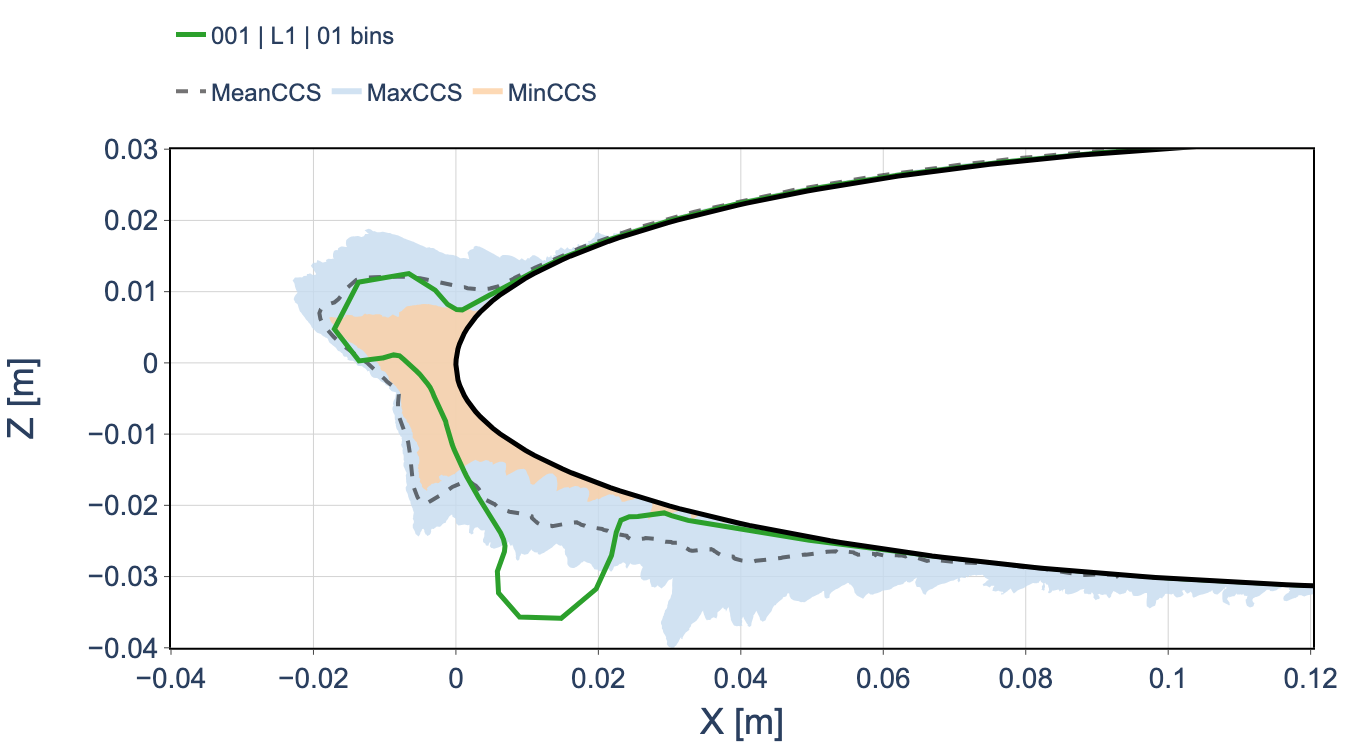
\includegraphics[width=\textwidth]{FIGURES/ICE_SHAPES/tc_naca0012_ae3932_finest_grid_multilayer_ice_shape_highest_bins.png}

    \vspace{0.05cm}

    {\scriptsize\textbf{AE3932}}
\end{column}

\begin{column}{0.50\textwidth}
    \centering
    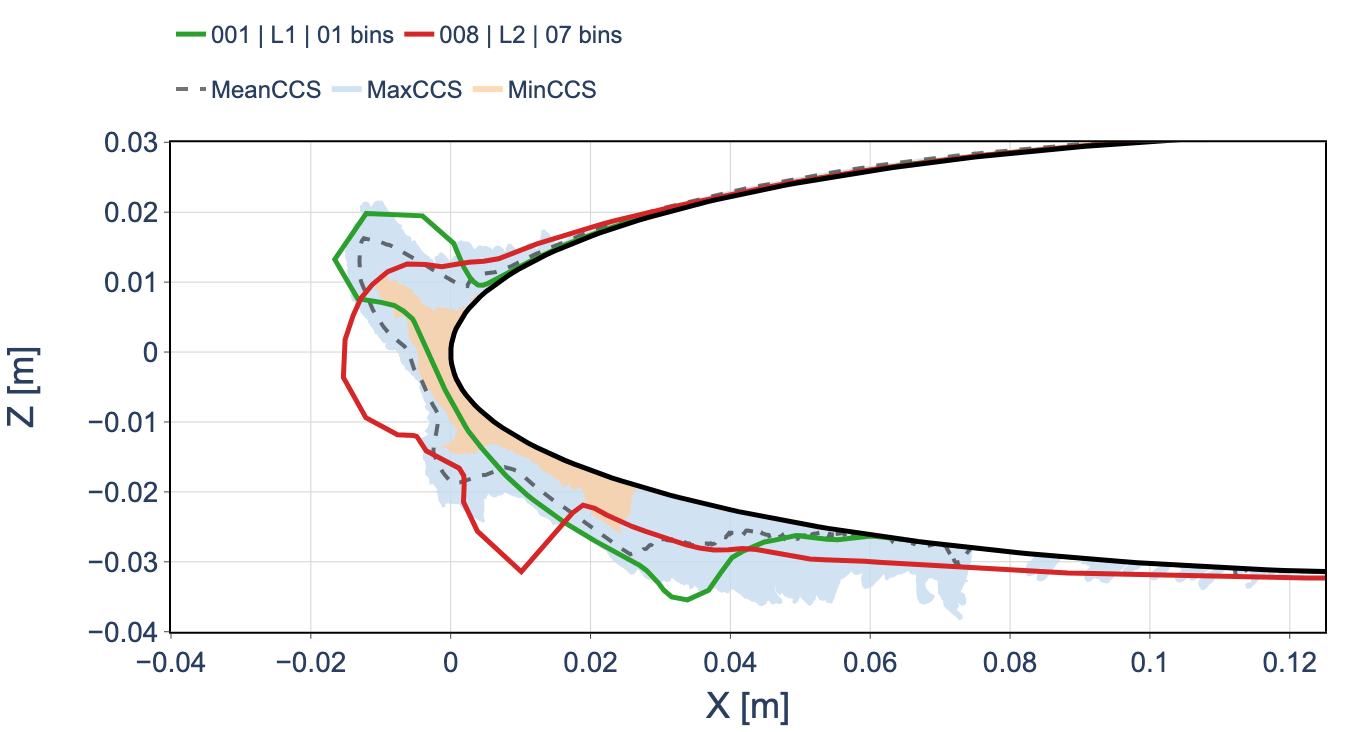
\includegraphics[width=\textwidth]{FIGURES/ICE_SHAPES/tc_naca0012_ae3933_finest_grid_multilayer_ice_shape_highest_bins.png}

    \vspace{0.05cm}

    {\scriptsize\textbf{AE3933}}
\end{column}

\end{columns}

\vspace{0.15cm}

\begin{block}{\scriptsize Observations}
\begin{itemize}
    \item Multilayer predictions suggest slight improvement, but the limited dataset prevents a conclusive assessment.
\end{itemize}
\end{block}

\end{frame}